\documentclass[UTF8]{ctexart}
\usepackage{amsmath,graphicx,enumerate,calc,alltt,capt-of,ifthen}
\usepackage[tikz]{mdframed}

\catcode`\<=\active \def<{
\fontencoding{T1}\selectfont\symbol{60}\fontencoding{\encodingdefault}}
\catcode`\>=\active \def>{
\fontencoding{T1}\selectfont\symbol{62}\fontencoding{\encodingdefault}}
\newcommand{\chapter}[1]{\medskip\bigskip

\noindent\textbf{\huge #1}}
\newcommand{\tmcodeinline}[2][]{{\ttfamily{#2}}}
\newcommand{\tmem}[1]{{\em #1\/}}
\newcommand{\tmop}[1]{\ensuremath{\operatorname{#1}}}
\newcommand{\tmsamp}[1]{\textsf{#1}}
\newcommand{\tmstrong}[1]{\textbf{#1}}
\newenvironment{enumeratenumeric}{\begin{enumerate}[1.] }{\end{enumerate}}
\newenvironment{tmcode}[1][]{\begin{alltt} }{\end{alltt}}
\mdfsetup{linecolor=black,linewidth=0.5pt,skipabove=0.5em,skipbelow=0.5em,hidealllines=true,innerleftmargin=0pt,innerrightmargin=0pt,innertopmargin=0pt,innerbottommargin=0pt}
\newcommand{\tmfloatcontents}{}
\newlength{\tmfloatwidth}
\newcommand{\tmfloat}[5]{
  \renewcommand{\tmfloatcontents}{#4}
  \setlength{\tmfloatwidth}{\widthof{\tmfloatcontents}+1in}
  \ifthenelse{\equal{#2}{small}}
    {\setlength{\tmfloatwidth}{0.45\linewidth}}
    {\setlength{\tmfloatwidth}{\linewidth}}
  \begin{minipage}[#1]{\tmfloatwidth}
    \begin{center}
      \tmfloatcontents
      \captionof{#3}{#5}
    \end{center}
  \end{minipage}}
\newmdenv[hidealllines=false,innertopmargin=1ex,innerbottommargin=1ex,innerleftmargin=1ex,innerrightmargin=1ex]{tmframed}

\begin{document}

\title{Glenda 内核设计手册}

\author{{\tmstrong{徐泽逸 汪子昊}}}

\maketitle

\section{摘要}

该文档将对我们设计的 Glenda 作详细的介绍。

Glenda 是一款使用 Rust 从零开发的、面向 RISC-V (rv64gc)
平台、分为宏内核与微内核两个版本的小型操作系统,宏内核的设计参考了
Plan9, Linux 和 xv6 的经典实现,微内核则主要参考了 seL4
的设计,同时我们也加入了一系列新的设计理念。

在这篇文档中,我们通过源代码讲解的方式来详细阐释我们的设计思路。同时,针对各个模块的实现,我们给出了充足的测试用例来证明其正确性。

Glenda 目前经历了近 400 次修改(以 commit
数计),总代码量:
\begin{itemize}
  \item 宏内核版本:约 8000 余行
  
  \item 微内核版本:TODO
\end{itemize}
截至 1 月 2 日,我们的系统完成情况如下所示:

$\begin{array}{|l|l|}
  \hline
  分支名 & 完成内容\\
  \hline
  \tmop{lab} 1 & 内核的基本输出功能和硬件解析,包括
  \tmop{UART} 驱动、 \tmop{Printk} 打印以及设备树解析器\\
  \hline
  \tmop{lab} 2 & 物理内存分配器和基于页表的虚拟内存管理\\
  \hline
  \tmop{lab} 3 & 中断处理机制,包括陷阱初始化、 \tmop{UART}
  中断处理以及时钟中断\\
  \hline
  \tmop{lab} 4 &
  进程管理模块,实现了基本的系统调用接口,并支持用户模式程序的加载与运行\\
  \hline
  \tmop{lab} 5 & 实现了 \tmop{mmap}
  内存映射系统调用,以及内核与用户空间之间的拷贝函数\\
  \hline
  \tmop{lab} 6 &
  实现了进程调度器和上下文切换逻辑,结合时钟中断实现了基本的多进程并发运行\\
  \hline
  \tmop{lab} 7 & 引入了 \tmop{VirtIO}
  块设备驱动,实现了缓冲区缓存和位图分配器\\
  \hline
  \tmop{lab} 8 &
  实现了文件系统的核心抽象,包括索引节点层、目录项缓存和路径解析逻辑\\
  \hline
  \tmop{lab} 9 &
  完善了进程生命周期管理以及用户态的文件系统调用接口,整合所有模块\\
  \hline
  \tmop{microkernel} & \tmop{Glenda} 的微内核实现\\
  \hline
\end{array}$

\

\

\

\

\

\

\

\

\

\

\

\

\

\chapter{Glenda 总览}

\subsection*{Glenda 宏内核总览}

\raisebox{0.0\height}{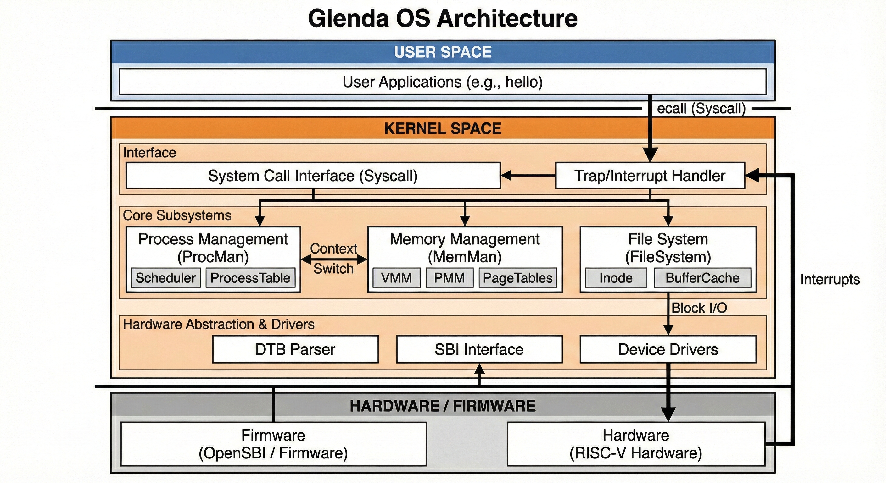
\includegraphics[width=14.874163715072806cm,height=8.107503607503608cm]{doc-1.pdf}}

Glenda 通过 Rust 语言的 Module
机制和文件目录结构来实现分层设计。大体上,Glenda
的内核架构分为:
\begin{itemize}
  \item Boot 与初始化模块:{\tmsamp{kernel/src/asm, kernel/src/init}}
  
  \item 中断与异常处理模块:{\tmsamp{kernel/src/irq,
  kernel/src/asm/vector.S}}
  
  \item 内存管理模块:{\tmsamp{kernel/src/mem}}
  
  \item 进程调度模块:{\tmsamp{kernel/src/proc}}
  
  \item 文件系统模块:{\tmsamp{kernel/src/fs, kernel/src/drivers}}
\end{itemize}

\subsection*{Glenda 微内核总览}

TODO

\subsection*{创新点}

Glenda 在完成了一个 OS
所必备的基本功能的基础上,还进行了一系列创新:

{\tmstrong{宏内核版本:}}
\begin{itemize}
  \item 实现了基于位图的调度器,能够在 $O (1)$
  时间复杂度内查找到可运行进程,提高了调度效率
  
  \item 利用 Rust
  的所有权机制和类型系统来增强内核的安全性
  
  \item 为 UART 模块引入了 Unicode 支持,支持 Emoji
  与多语言处理
  
  \item 实现了 COW 策略
  
  \item 实现了类似 UNIX 下的多级索引文件结构
  
  \item 实现了 DTB
  探测与解析,不需要硬编码硬件,增加了内核的可移植性
  
  \item 提供了一个初步的 shell 环境,并实现了 Lisp
  解释器/文本编辑器等应用
\end{itemize}
{\tmstrong{微内核版本:}}

TODO (这里应该可以加 Buddy System,
我记得微内核好像有,总之炫酷的东西写里面就行)

\subsection*{运行方法}

Glenda 使用了自制的 xtask
实现,将构建系统、磁盘镜像生成器与测试编排工具打包成了一个可以直接由
Cargo
驱动的工具,使得无需安装额外的非标准工具即可构建出带有预置数据的可启动镜像成为可能。

Glenda 的 xtask 有以下功能:

\begin{center}
  \raisebox{0.0\height}{\includegraphics[width=10.411911321002231cm,height=7.020972714154532cm]{doc-2.pdf}}
\end{center}
\begin{itemize}
  \item {\tmsamp{build}}:构建项目
  
  \item {\tmsamp{run}}:使用 QEMU 运行内核,可以用{\tmsamp{
  --cpus}} 来修改启动 hart 数量 (最大为 8,默认为 4),用
  {\tmsamp{--mem}} 来修改启动内存 (默认 512MB)
  
  \item {\tmsamp{test}}: 运行内核的测试点(参数同
  {\tmsamp{run}})
  
  \item {\tmsamp{gdb}}: 使用 GDB/LLDB 远程调试内核
  
  \item {\tmsamp{mkfs}}:生成磁盘镜像
  
  \item {\tmsamp{--release}}:启用编译优化
  
  \item {\tmsamp{--features}}:启用额外特性 (例如 Unicode 支持)
\end{itemize}

\subsubsection{运行命令}

{\tmsamp{{\tmstrong{\begin{center}
  GLENDA\_RICH\_MKFS=1 cargo xtask test
\end{center}}}}}

\

\chapter{Boot 模块}

\subsection*{功能介绍}

boot 模块主要涉及 {\tmsamp{kernel/src/asm}}
中的汇编启动代码和{\tmsamp{ kernel/src/main.rs}} 中的 Rust
入口函数。用于完成系统的底层环境搭建、内核启动以及各个子系统的初始化工作

\subsection*{实现分析}

在 Glenda 的启动流程中,系统上电后首先由 OpenSBI(M
模式)接管硬件,完成基础硬件初始化后,跳转到 S
模式下的内核入口地址 0x80200000(由
{\tmsamp{kernel/src/linker.ld}} 定义)

\subsubsection{汇编入口}

内核的执行始于 {\tmsamp{\_start}}
标签。该汇编程序的主要任务是为当前 CPU Hart
分配启动栈。考虑到多核启动的安全性,Glenda
预定义了最大启动核心数为 8,汇编代码会首先检查当前
hartid 是否在有效范围内(0-7),如果合法,它会根据 hartid
计算出每个核心在 {\tmsamp{.bss}} 段中预留的
{\tmsamp{boot\_stack}} 的偏移位置,设置好栈指针 sp;若 hartid
超过限制,则会将其栈指针重定向至安全区域以防止内存越界。然后通过
{\tmsamp{tail glenda\_main}} 跳转到 Rust 语言编写的内核主函数。

\begin{tmcode}
 

\end{tmcode}

\subsubsection{内核主函数}

{\tmsamp{glenda\_main}} 函数是内核的高级语言入口。根据
$\tmop{RISC} - V \tmop{Linux} \tmop{Kernel} \tmop{Boot}
\tmop{Requirements}^{[1]}$,它接收 {\tmsamp{hartid}} 和设备树指针
{\tmsamp{dtb}} 作为参数,并调用 {\tmsamp{init}}
函数进行系统初始化。

\subsubsection{系统初始化}

初始化过程使用了 {\tmsamp{spin::Once}}
保证全局资源只被初始化一次,同时兼顾了多核启动的同步:

Glenda 由第一个竞争到的 CPU 核心负责初始化设备树
(DTB)、UART 驱动、物理内存管理 (PMEM)、全局中断控制器
(IRQ)、文件系统 (VirtIO/Buffer) 等共享资源。

同时,所有核心都会执行 {\tmsamp{irq::init\_hart}}
来开启本地中断、{\tmsamp{vm::switch\_to\_kernel}}
来加载内核页表,以及 {\tmsamp{hart::init}}
来初始化每个核心的私有数据结构。

\begin{tmframed}
  \begin{tmcode}[cpp]
  \#[unsafe(no_mangle)]
pub extern "C" fn glenda_main(hartid: usize, dtb: *const u8) -> ! \{
    init(hartid, dtb);

    #[cfg(feature = "tests")]
    \{
        tests::test(hartid);
    \}

    if hartid == 0 \{
        // Enter kernel shell on boot
        shell::run();
    \}

    printk!("\{\}Hart \{\} entering main loop\{\}\textbackslash n", ANSI_BLUE, hartid, ANSI_RESET);
    loop \{
        wfi();
    \}
\}
  \end{tmcode}
\end{tmframed}

\subsubsection{测试}

在完成了所有的初始化后,每个 cpu
都会打印一条消息表明成功启动:

\begin{center}
  \raisebox{0.0\height}{\includegraphics[width=7.437081857536403cm,height=3.176505312868949cm]{doc-3.pdf}}
\end{center}

\

\

\

\

\

\

\chapter{中断处理模块}

\subsection*{功能介绍}

中断是系统实现用户接口和硬件访问的重要工具,当中断或异常发生时,处理器会暂停当前正在执行的任务,保存其状态,并跳转到专门的中断处理程序来处理这些事件。这种机制确保了系统的稳定性和安全性。在
Glenda 中,中断模块位于 {\tmsamp{kernel/src/irq/trap}} 中。

\subsection*{中断处理的过程}

中断处理中,Glenda 分为 {\tmsamp{kernel}} 态和 {\tmsamp{user}}
态分别处理。

核心处理函数分别为
{\tmsamp{trap\_kernel\_handler}}(处理内核态中断/异常)和
{\tmsamp{trap\_user\_handler}}(处理用户态陷阱)。此外,还有
{\tmsamp{kernel\_vector}} 和 {\tmsamp{user\_vector}}(位于
{\tmsamp{trampoline.S}})这两个汇编入口函数,分别用于保存/恢复
CPU 状态并跳转到相应的 Rust 处理逻辑。

\subsubsection{M 模式下的中断处理}

在 Glenda 中,M 模式下的中断处理主要通过 {\tmsamp{vector.S}}
中的 {\tmsamp{timer\_vector}} 处理时钟中断。

OpenSBI 或类似的固件引导后,时钟中断会触发 M
模式下的陷阱。{\tmsamp{{\tmsamp{timer\_vector}}}} 会更新
{\tmsamp{mtimecmp}} 以设置下一次时钟触发时间,并触发一个 S
模式的软件中断 (SSIP),从而将时钟事件转发给 S
模式内核处理。

\subsubsection{S 模式下的中断处理}

S 模式下的中断处理根据来源有所不同,由 {\tmsamp{stvec}}
寄存器指向不同的入口地址:

{\tmstrong{内核态陷阱:}}
\begin{itemize}
  \item 当内核代码执行过程中发生中断或异常,CPU 跳转到
  {\tmsamp{kernel\_vector}},它将所有通用寄存器保存到内核栈上,然后调用
  {\tmsamp{trap\_kernel\_handler(ctx: \&mut
  TrapContext)}}。{\tmsamp{trap\_kernel\_handler}} 根据 {\tmsamp{scause}}
  分发处理。
  
  \begin{tmframed}
    \begin{tmcode}[cpp]
    /// S-mode 
///  kernel_vector 
/// # 
/// - `ctx`: 
#[unsafe(no_mangle)]
pub extern "C" fn trap_kernel_handler(ctx: &mut TrapContext) \{
    interrupt::enter();
    let sc = scause::read();
    let epc = sepc::read();
    let tval = stval::read();
    let sstatus_bits = sstatus::read().bits();

    match sc.cause() \{
        Trap::Exception(e) => \{
            exception_handler(e, epc, tval, sstatus_bits, ctx);
        \}
        Trap::Interrupt(i) => \{
            interrupt_handler(i, epc, tval, sstatus_bits, ctx);
        \}
    \}
    interrupt::exit();
\}
    \end{tmcode}
  \end{tmframed}
  
  \item {\tmstrong{异常:}}通过 {\tmsamp{exception\_handler}}
  处理,如缺页异常,则调用 {\tmsamp{ustack\_grow}}
  处理用户栈增长或打印错误信息并 Panic。
  
  \begin{tmframed}
    \begin{tmcode}[cpp]
    /// 
fn exception_handler(
    e: usize,
    epc: usize,
    tval: usize,
    sstatus_bits: usize,
    ctx: &mut TrapContext,
) \{
    // 8: Environment call from U-mode
    if e == 8 \{
        user::syscall_handler(ctx);
        unsafe \{
            sepc::write(epc.wrapping_add(4));
        \}
        return;
    \}

    // 13: Load Page Fault, 15: Store/AMO Page Fault
    if e == 13 || e == 15 \{
        let p = proc::current_proc();
        if p.ustack_grow(tval).is_ok() \{
            return;
        \}
    \}
    printk!(
        "\{\}TRAP(Exception)\{\}: code=\{\} (\{\}); epc=0x\{:x\}, tval=0x\{:x\},
         sstatus=0x\{:x\}\textbackslash n",
        ANSI_RED,
        ANSI_RESET,
        e,
        EXCEPTION_INFO.get(e).unwrap_or(&"Unknown Exception"),
        epc,
        tval,
        sstatus_bits
    );
    panic!("Kernel panic due to exception");
\}
    \end{tmcode}
  \end{tmframed}
  
  \item {\tmstrong{中断:}}通过 {\tmsamp{interrupt\_handler}}
  处理,包括 S 模式时钟中断$^{[见后文]}$(调用
  {\tmsamp{timer::update}} 和
  {\tmsamp{scheduler::yield\_proc}})、外部中断(PLIC,处理 UART 和
  VirtIO)等。
  
  \begin{tmframed}
    \begin{tmcode}[cpp]
     1 /// 
 2 fn interrupt_handler(
 3     e: usize,
 4     epc: usize,
 5     tval: usize,
 6     sstatus_bits: usize,
 7     _ctx: &mut TrapContext,
 8 ) \{
 9     match e \{
10         9 => external_handler(),
11         // S-mode timer interrupt
12         5 => timer_handler_stip(sstatus_bits),
13         // S-mode software interrupt
14         1 => timer_handler_ssip(sstatus_bits),
15         _ => \{
16             printk!(
17                 "\{\}TRAP(Interrupt)\{\}: code=\{\} (\{\}); epc=0x\{:x\},
18                  tval=0x\{:x\}, sstatus=0x\{:x\}\textbackslash n",
19                 ANSI_YELLOW,
20                 ANSI_RESET,
21                 e,
22                INTERRUPT_INFO.get(e).unwrap_or(&"Unknown Interrupt"),
23                 epc,
24                 tval,
25                 sstatus_bits
26             );
27         \}
28     \}
29 \}
    \end{tmcode}
  \end{tmframed}
\end{itemize}
{\tmstrong{用户态陷阱:}}

当在用户态触发陷阱后,CPU 跳转到
{\tmsamp{user\_vector}}(位于 {\tmsamp{trampoline.S}})

这是一段特殊的代码,是映射在内核和用户空间的高地址共享区域
{\tmsamp{TRAMPOLINE}}

\subsubsection{返回用户态}

处理完成后,通过 {\tmsamp{trap\_user\_return}} 函数和
{\tmsamp{user\_return}} 汇编代码返回用户态:

首先使用 {\tmsamp{sstatus::clear\_sie}} 关闭 S 模式中断,将
{\tmsamp{stvec}} 重新指向 {\tmsamp{user\_vector}},设置
{\tmsamp{sstatus::spp}} 为 User 模式,然后跳转到
{\tmsamp{user\_return}},通过 {\tmsamp{csrw satp, a1}}
切换回用户页表,从 TrapFrame
中恢复所有通用寄存器。最后执行 sret 指令,切换回 U
模式并跳转到 sepc 指定的地址继续执行用户程序。

\subsection*{时钟中断}

\subsubsection{原理}

在 RISC-V 架构中,系统时间由 {\tmsamp{mtime}} 寄存器维护,而
{\tmsamp{mtimecmp}}
寄存器用于设置下一次中断触发的时间点。当 {\tmsamp{mtime >=
mtimecmp}} 时,硬件会产生一个 M 模式的时钟中断。

\begin{center}
  \raisebox{0.0\height}{\includegraphics[width=13.386740784468058cm,height=8.00490292535747cm]{doc-4.pdf}}
\end{center}

由于 Glenda 运行在 S 模式,无法直接访问 M
模式的寄存器。因此,Glenda 借助 OpenSBI
提供的标准接口来实现时钟管理。OpenSBI 运行在 M
模式,它会捕获硬件时钟中断,并通过软件注入的方式,将其转化为
S 模式下的时钟中断或 S 模式软件中断传递给内核。

\subsubsection{初始化过程}

Glenda 的时钟中断初始化流程主要在 {\tmsamp{irq::init\_hart}} 和
{\tmsamp{interrupt::enable\_s}} 中完成:

首先,Glenda 会设置中断向量表,将 {\tmsamp{stvec}}
寄存器指向 {\tmsamp{kernel\_vector}} 的地址。这确保了当 S
模式中断发生时,CPU
能跳转到正确的内核处理入口;然后,内核会开启 S
模式中断,通过设置 sie 寄存器来开启特定的中断源:

\begin{tmframed}
  \begin{tmcode}[cpp]
     1     unsafe \{
   2         sie::set_ssoft();   //  S 
   3         sie::set_stimer();  //  S 
   4         super::timer::start(hartid); // 
   5     \}
  \end{tmcode}
\end{tmframed}

紧接着,{\tmsamp{timer::start}} 会调用
{\tmsamp{timer::program\_next\_tick()}},通过 SBI
接口设置中断触发的时间点。

\subsubsection{时间中断处理函数}

如先前所述,当 OpenSBI 转发的时钟中断到达内核时,会触发
{\tmsamp{trap\_kernel\_handler}}。根据中断类型,最终调用
{\tmsamp{timer\_handler\_stip}} 或 {\tmsamp{timer\_handler\_ssip}}

这两个处理函数的核心逻辑如下:
\begin{itemize}
  \item 调用 {\tmsamp{timer::update()}},原子递增全局计数器
  {\tmsamp{SYS\_TICKS}}
  
  \item 调用
  {\tmsamp{scheduler::wakeup}},检查是否有进程正在睡眠等待当前的时间点
  
  \item 调用
  {\tmsamp{timer::program\_next\_tick()}},计算下一次中断时间(当前时间
  + {\tmsamp{INTERVAL}}),并再次通过 SBI 接口设置硬件
  
  \item 检查 sstatus 确保允许抢占后,调用
  {\tmsamp{scheduler::yield\_proc()}},强制当前进程放弃
  CPU,从而实现时间片轮转调度,确保了系统不会被某个单一进程长期霸占
\end{itemize}

\subsection*{系统调用}

用户程序通过执行特定的指令(ecall)发起系统调用请求。

\subsubsection{内核处理请求}

如先前所述,{\tmsamp{trap\_kernel\_handler}} 会读取 {\tmsamp{scause}}
寄存器判断陷阱原因。如果是系统调用(Exception Code 为
8),则进入 {\tmsamp{exception\_handler}} 并调用
{\tmsamp{user::syscall\_handler(ctx)}}

{\tmsamp{syscall\_handler}} 最终调用
{\tmsamp{syscall::dispatch(ctx)}},在 {\tmsamp{kernel/src/syscall/mod.rs}}
中,Glenda 使用 Rust 的 match
通过模式匹配来分发系统调用,而不是像 C
语言内核那样查表。系统调用号存储在 a7
寄存器中,参数通常在 a0-a5 中:

\begin{tmframed}
  \begin{tmcode}[cpp]
      1 // kernel/src/syscall/mod.rs
    2 
    3 pub fn dispatch(ctx: &mut TrapContext) -> usize \{
    4     match ctx.a7 \{
    5         SYS_HELLOWORLD => helloworld::sys_helloworld(),
    6         SYS_COPYOUT => copy::sys_copyout(ctx),
    7         SYS_BRK => brk::sys_brk(ctx),
    8         SYS_MMAP => mmap::sys_mmap(ctx),
    9         SYS_FORK => proc::sys_fork(),
   10         SYS_WAIT => proc::sys_wait(ctx),
   11         SYS_EXIT => proc::sys_exit(ctx),
   12         SYS_OPEN => fs::sys_open(ctx),
   13         SYS_READ => fs::sys_read(ctx),
   14         SYS_WRITE => fs::sys_write(ctx),
   15         // ......
   16         n => \{
   17             printk!("SYSCALL: unknown number \{\}\textbackslash n", n);
   18             usize::MAX
   19         \}
   20     \}
   21 \}
  \end{tmcode}
\end{tmframed}

\subsubsection{返回用户状态}

在内核完成系统调用处理后,控制权流向
trap\_user\_return,该函数的原理已在上文进行过解释,这里不再赘述,只给出代码实现:

\begin{tmframed}
  \begin{tmcode}[cpp]
      1 // kernel/src/irq/trap/user.rs
    2 
    3 #[unsafe(no_mangle)]
    4 pub extern "C" fn trap_user_return(_ctx: &mut TrapFrame) \{
    5     
    6     //  user_vector
    7     stvec::write(Stvec::new(user_vec_addr, stvec::TrapMode::Direct));
    8 
    9     //  sepc  PC
   10     sepc::write(ctx.kernel_epc);
   11
   12     sstatus::set_spp(sstatus::SPP::User);
   13      
   14     let user_return_fn: extern "C" fn(u64, u64) -> ! = unsafe \{ mem::transmute(user_ret_addr) \};
   15     user_return_fn(user_tf_va as u64, user_satp)
   16 \}
  \end{tmcode}
\end{tmframed}

\subsection*{外设中断}

Glenda 中的外设中断基于
PLIC,主要处理两类设备:一类是负责串口通信的
UART,另一类是负责磁盘读写的 VirtIO。

当 CPU 收到 S 模式外设中断(Trap ID 9)时,会调用{\tmsamp{
external\_handler()}}。该函数负责向 PLIC
查询当前优先级最高的中断源,并分发给对应的驱动程序处理,最后通知
PLIC 中断已处理完毕。

\begin{tmframed}
  \begin{tmcode}[cpp]
      1 // kernel/src/irq/trap/kernel.rs
    2 
    3 pub fn external_handler() \{
    4     let hartid = hart::getid();
    5     // 
    6     let id = plic::claim(hartid);
    7     
    8     match id \{
    9         0 => return,
   10         plic::UART_IRQ => \{
   11             //  UART 
   12             drivers::uart::irq::handler();
   13         \},
   14         plic::VIRTIO0_IRQ => \{
   15             //  VirtIO 
   16             drivers::virtio::disk::intr();
   17         \},
   18         _ => \{
   19             panic!("Unexpected interrupt id \{\} on hart \{\}", id, hartid);
   20         \}
   21     \}
   22 
   23     plic::complete(hartid, id);
   24 \}
  \end{tmcode}
\end{tmframed}

\subsection*{测试}

\subsubsection{时钟滴答测试}

Glenda
使用这个测试点判断时钟中断能否正确触发,以及多核环境下中断能否被正确处理:

\begin{center}
  \raisebox{0.0\height}{\includegraphics[width=7.437081857536403cm,height=15.632067427521973cm]{doc-5.pdf}}
\end{center}

\subsubsection{UART 并发输出测试}

虽然主要测试 UART,但同时也隐式验证了 PLIC
和自旋锁在中断环境下的稳定性

\begin{center}
  \raisebox{0.0\height}{\includegraphics[width=7.437081857536403cm,height=15.33007018234291cm]{doc-6.pdf}}
\end{center}

\

\chapter{内存管理模块}

\subsection*{功能介绍}

内存管理系统是操作系统中负责分配、回收和管理计算机内存的关键组件。它通过为进程分配合适的内存空间,确保每个进程能够高效运行,同时避免内存冲突和浪费。Glenda
的虚拟地址管理基于 RISC-V 的 Sv39
模式,即虚拟地址空间大小为 $2^{39}$-1 个字节。

\subsection*{物理内存的管理}

\subsubsection{物理内存布局}

Glenda
采用了将物理内存分割为不同用途区域的策略,以提高内存管理的灵活性和安全性。物理内存的布局主要基于
QEMU Virt
平台和链接脚本定义的符号。因此,我们可以将物理内存大致分为下面三部分:
\begin{enumeratenumeric}
  \item 内核镜像区
  
  从 0x80200000 开始,包含了内核的代码段
  (.text)、只读数据段 (.rodata)、数据段 (.data) 和 BSS 段
  (.bss)。这部分内存在系统启动加载时已被占用,不可作为空闲页分配
  
  \item 内核分配区
  
  紧接在内核 BSS
  段之后,延伸至指定的内核页数限制({\tmsamp{KERN\_PAGES}},默认为
  8192 页,即
  32MB)。这部分内存专门用于内核数据结构(如内核页表、内核栈、进程控制块等)的动态分配。此区域的目的是为了保证内核在高负载下仍有稳定的内存供应,且方便实现
  1:1 的直接映射。
  
  \item 用户分配区
  
  从内核分配区结束位置开始,一直延伸到物理内存的末尾。这部分内存是最大的,用于分配用户进程的页面(代码、数据、堆、栈)以及磁盘缓冲区等。
\end{enumeratenumeric}
\begin{center}
  \raisebox{0.0\height}{\includegraphics[width=14.874163715072806cm,height=8.123573396300669cm]{doc-7.pdf}}
\end{center}

Glenda 在 {\tmsamp{kernel/src/mem/pmem.rs}} 中定义物理页的大小
PGSIZE 为 4096
Bytes,这样问题就从管理连续的地址空间转化成了管理有限个独立的物理页。为了便于物理页的插入和移出,Glenda
使用单向链表来维护空闲页面。

\begin{tmframed}
  \begin{tmcode}[cpp]
      1 // 
    2 #[repr(C)]
    3 struct FreePage \{
    4     next: Option<NonNull<FreePage>>,
    5 \}
    6 
    7 // 
    8 #[derive(Clone, Copy)]
    9 struct RegionInner \{
   10     head: Option<NonNull<FreePage>>, 
   11     allocable: usize,
   12 \}
   13 
   14 // 
   15 struct AllocRegion \{
   16     bounds: OnceCell<RegionBounds>,
   17     inner: Mutex<RegionInner>,
   18 \}
   19 
   20 static KERNEL_REGION: AllocRegion = AllocRegion::new();
   21 static USER_REGION: AllocRegion = AllocRegion::new();
  \end{tmcode}
\end{tmframed}

\subsubsection{物理内存的初始化}

Glenda 的物理内存初始化逻辑位于 {\tmsamp{initialize\_regions}}
函数中。它会计算内核镜像结束的位置,然后将剩余的可用物理内存划分为内核专用区和用户专用区。

\begin{tmframed}
  \begin{tmcode}[cpp]
      1 pub fn initialize_regions(hartid: usize) \{
    2     // 
    3     let alloc_begin = addr_of_mut!(__alloc_start) as PhysAddr;
    4     let alloc_end = mem_end; //  DTB Parser 
    5     
    6     // 
    7     let kernel_split = align_up(alloc_begin + KERN_PAGES * PGSIZE);
    8 
    9     unsafe \{
   10         // 
   11         KERNEL_REGION.init(alloc_begin, kernel_split);
   12         // 
   13         USER_REGION.init(kernel_split, alloc_end);
   14     \}
   15     
   16     // ...
   17 \}
   18 
   19 impl AllocRegion \{
   20     unsafe fn init(&self, begin: PhysAddr, end: PhysAddr) \{
   21         // 
   22         let mut head: Option<NonNull<FreePage>> = None;
   23         let mut current = begin;
   24         while current + PGSIZE <= end \{
   25             let page = current as *mut FreePage;
   26             (*page).next = head;
   27             head = NonNull::new(page);
   28             current += PGSIZE;
   29         \}
   30         // ... 
   31     \}
   32 \}
  \end{tmcode}
\end{tmframed}

初始化过程同样是分区域进行的。通过这种方式,内核和用户的物理内存被清晰地分隔,并且每个区域都有独立的锁和链表,确保在后续高并发的内存分配和回收过程中减少锁竞争并防止冲突。

\subsubsection{物理内存的分配与回收}

物理内存的分配与回收由 {\tmsamp{pmem::alloc}} 和
{\tmsamp{pmem::free}}
函数实现。为了支持内核与用户内存隔离,这两个函数通过
{\tmsamp{for\_kernel}} 参数或根据物理地址范围自动选择操作
{\tmsamp{KERNEL\_REGION}} 还是 {\tmsamp{USER\_REGION}}。
\begin{itemize}
  \item {\tmsamp{alloc(for\_kernel: bool)}}:根据 {\tmsamp{for\_kernel}}
  标志选择对应的内存区域分配器,返回一个未使用的、内容已清零的物理页指针。如果分配失败,则触发
  Panic。成功分配时,会通过全局原子数组 {\tmsamp{PAGE\_REF}}
  将该页面的引用计数设为 1。
  
  \item {\tmsamp{free(addr: PhysAddr,
  ...)}}:首先将指定物理页的引用计数减
  1。只有当引用计数降至 0
  时,才真正将其归还给对应的内存区域链表。这种机制是实现共享内存和未来
  COW 的基础。
\end{itemize}
为了保证操作的高效性 ($O (1)$复杂度),Glenda
始终从链表头部取出页面进行分配,归还时也使用头插法将页面插回链表。

\begin{tmframed}
  \begin{tmcode}[cpp]
   1 // kernel/src/mem/pmem.rs
 2 
 3 pub fn alloc(for_kernel: bool) -> *mut u8 \{
 4     let region = if for_kernel \{ &KERNEL_REGION \} else \{ &USER_REGION \};
 5 
 6     match region.allocate() \{
 7         Some(ptr) => ptr,
 8         None => panic!("pmem_alloc: region exhausted"),
 9     \}
10 \}
11 
12 fn allocate(&self) -> Option<*mut u8> \{
13     let head_ptr = \{
14         let mut inner = self.inner.lock();
15         let head = inner.head?;
16         let next = unsafe \{ (*head.as_ptr()).next \};
17         inner.head = next;
18         inner.allocable -= 1;
19         head
20     \};
21 
22     let p = head_ptr.as_ptr() as *mut u8;
23     let idx = pa_to_index(p as usize);
24     
25     if PAGE_REF[idx].fetch_add(1, Ordering::SeqCst) != 0 \{
26         panic!("pmem_alloc: ref count corrupted");
27     \}
28     
29     unsafe \{ ptr::write_bytes(p, 0, PGSIZE) \};
30     Some(p)
31 \}
32 
33 pub fn free(addr: PhysAddr, _for_kernel: bool) \{
34     let region = if KERNEL_REGION.contains(addr) \{
35         &KERNEL_REGION
36     \} else if USER_REGION.contains(addr) \{
37         &USER_REGION
38     \} else \{
39         panic!("pmem_free: address out of bounds");
40     \};
41 
42     let idx = pa_to_index(addr);
43     let old = PAGE_REF[idx].fetch_sub(1, Ordering::SeqCst);
44     
45     if old > 1 \{
46         return;
47     \}
48 
49     region.free(addr);
50 \}
51 
52 fn free(&self, addr: PhysAddr) \{
53     let mut inner = self.inner.lock();
54     unsafe \{
55         let page = addr as *mut FreePage;
56         (*page).next = inner.head;
57         inner.head = NonNull::new(page);
58     \}
59     inner.allocable += 1;
60 \}
  \end{tmcode}
\end{tmframed}

\subsubsection{COW}

在上面的代码中已经实现了支持引用计数的物理内存管理器。为了实现高效的
COW 机制,还需要在页表复制逻辑和 PTE
定义上做进一步的工作。

在 {\tmsamp{fork}} 系统调用中,Glenda 不再通过
{\tmsamp{PageTable::copy}}
完全深拷贝父进程的物理内存,而是让父子进程共享同一物理内存。具体的做法是:遍历父进程的内存空间,如果遇到可写的用户页,则将其在父子进程的页表中都标记为只读(清除
{\tmsamp{PTE\_W}}),并设置 {\tmsamp{PTE\_COW}}
标志,同时增加物理页的引用计数。当任一进程尝试写入时,触发
Store Page
Fault,由异常处理程序执行实际的内存分配和复制。

\begin{tmframed}
  \begin{tmcode}[cpp]
   1 if (flags & PTE_U) != 0 \{
 2     match pmem::get_region(pa) \{
 3         Some(for_kernel) if !for_kernel => \{
 4             if (flags & PTE_W) != 0 \{
 5                 let cow_flags = (flags & !PTE_W) | pte::PTE_COW;
 6                 unsafe \{ *pte_ptr = pa_to_pte(pa, cow_flags); \}
 7                 if !dst_pt.map(va, pa, PGSIZE, cow_flags) \{ return Err(UvmError::MapFailed); \}
 8             \} else \{
 9                 if !dst_pt.map(va, pa, PGSIZE, flags) \{ return Err(UvmError::MapFailed); \}
10             \}
11             pmem::inc_ref(pa);
12         \}
13         // ...
14     \}
15 \}
  \end{tmcode}
\end{tmframed}

除了将 PTE 设置为只读外,还需要通过 RISC-V PTE
的预留位来标记该页面为 COW
页面,以便在缺页异常处理中与普通的只读页面(如代码段)区分开:

\begin{tmframed}
  \begin{tmcode}[cpp]
     1 // kernel/src/mem/pte.rs
   2 
   3 pub const PTE_D: usize = 1 << 7;   // Dirty
   4 pub const PTE_COW: usize = 1 << 8; // COW
  \end{tmcode}
\end{tmframed}

\subsubsection{PageFault 处理}

至此,Glenda 基本实现了
{\tmsamp{COW}},接下来要做的就是处理写时复制时发生的
{\tmsamp{Page Fault}}。这里只需要处理{\tmsamp{ scause == 15 (Store/AMO
Page Fault)}} 的情况,因为 13 是 Load Page Fault,而 COW
的只读保护不会引起读错误。

Glenda 定义了核心处理函数 {\tmsamp{handle\_co}}w,其逻辑集成在
{\tmsamp{kernel/src/mem/uvm.rs}} 中。当进程尝试写入 COW
页面时,会触发异常,内核分配新物理页,复制原数据,并更新页表:

\begin{tmframed}
  \begin{tmcode}[cpp]
      1 // kernel/src/mem/uvm.rs
    2 
    3 pub fn handle_cow(pt: &mut PageTable, va: VirtAddr) -> Result<(), UvmError> \{
    4     let va = align_down(va);
    5     // 
    6     let pte_ptr = pt.lookup(va).ok_or(UvmError::OutOfRange)?;
    7     let pte = unsafe \{ *pte_ptr \};
    8 
    9     // 
   10     if !pte::is_valid(pte) || (pte::get_flags(pte) & PTE_U) == 0 \{
   11         return Err(UvmError::Fault);
   12     \}
   13     
   14     //  COW 
   15     if (pte::get_flags(pte) & pte::PTE_COW) == 0 \{
   16          return Err(UvmError::Fault);
   17     \}
   18 
   19     let old_pa = pte_to_pa(pte);
   20     let old_flags = pte::get_flags(pte);
   21 
   22     // 
   23     let new_pa_ptr = pmem::alloc(false);
   24     let new_pa = new_pa_ptr as usize;
   25     if new_pa == 0 \{
   26         return Err(UvmError::NoMem);
   27     \}
   28 
   29     // 
   30     unsafe \{
   31         ptr::copy_nonoverlapping(old_pa as *const u8, new_pa as *mut u8, PGSIZE);
   32     \}
   33 
   34     //  PTE COW 
   35     let new_flags = (old_flags | PTE_W) & !pte::PTE_COW;
   36     unsafe \{
   37         *pte_ptr = pte::pa_to_pte(new_pa, new_flags);
   38     \}
   39 
   40     //  TLB CPU 
   41     unsafe \{ riscv::asm::sfence_vma_all(); \}
   42 
   43     // 
   44     //  0
   45     pmem::free(old_pa, false);
   46 
   47     Ok(())
   48 \}
  \end{tmcode}
\end{tmframed}

有了这个函数,便能在 {\tmsamp{trap\_kernel\_handler}} 中增加对
Page Fault 的处理了。当捕获到 {\tmsamp{Exception Code 15}}
时,首先尝试按 {\tmsamp{COW}} 处理,如果失败(如非
{\tmsamp{COW}}
页面或内存不足),则进一步判断是否为栈增长或 Panic:

\begin{tmframed}
  \begin{tmcode}[cpp]
      1 // kernel/src/irq/trap/kernel.rs
    2 
    3 // 13: Load Page Fault, 15: Store/AMO Page Fault
    4 if e == 13 || e == 15 \{
    5     let p = proc::current_proc();
    6     
    7     //  COW 
    8     if e == 15 \{
    9         let pt = unsafe \{ &mut *(p.root_pt_pa as *mut PageTable) \};
   10         if uvm::handle_cow(pt, tval).is_ok() \{
   11             return;
   12         \}
   13     \}
   14     
   15     // 
   16     if p.ustack_grow(tval).is_ok() \{
   17         return;
   18     \}
   19 \}
  \end{tmcode}
\end{tmframed}

\subsection*{虚拟内存的管理}

\subsubsection{内核页表布局}

Glenda 的内核页表设计参考了 xv6,采用 Sv39
模式。内核页表的绝大多数表项是直接映射到物理内存的,即虚拟地址等于物理地址。这包括内核代码段、数据段以及
I/O 设备内存。

同时,KSTACK和 TRAMPOLINE/TRAPFRAME
等用户页表和内核页表所共有的关键结构不是直接映射,它们被映射在虚拟地址空间的最高位,以便在上下文切换时保持地址固定。这种布局确保了内核在处理中断和系统调用时能够高效地访问关键数据结构。

\begin{center}
  \raisebox{0.0\height}{\includegraphics[width=14.874163715072806cm,height=9.53761642398006cm]{doc-8.pdf}}
\end{center}

\subsubsection{用户页表布局}

\begin{center}
  \raisebox{0.0\height}{\includegraphics[width=14.874163715072806cm,height=9.456660763478945cm]{doc-9.pdf}}
\end{center}

\subsection*{测试}

Glenda 为内存管理模块编写了全面的 Rust
集成测试,主要包含物理内存并发测试和虚拟内存映射测试两部分。这些测试在内核启动阶段通过
{\tmsamp{tests::test}} 入口执行。

\subsubsection{物理内存的分配}

该测试旨在验证多核环境下物理内存分配器的正确性和并发安全性。

\begin{center}
  \raisebox{0.0\height}{\includegraphics[width=7.437081857536403cm,height=3.0855962219598583cm]{doc-10.pdf}}
\end{center}

\subsubsection{页表的实现}

\begin{itemize}
  \item vm\_mapping\_test:
  
  该测试验证虚拟内存管理 (vm) 和页表操作 (PageTable)
  的正确性
  
  \item vm\_func\_test
  
  测试跨越多级页表、大跨度地址以及虚拟地址顶端的映射情况
\end{itemize}
\begin{center}
  \raisebox{0.0\height}{\includegraphics[width=7.437081857536403cm,height=13.912780401416764cm]{doc-11.pdf}}
\end{center}

\chapter{进程调度模块}

\subsection*{功能介绍}

进程调度模块是操作系统中负责管理和分配 CPU
使用权的核心组件。在 Glenda
中,调度算法已从传统的线性扫描进化为基于位图的 $O (1)$
调度算法。结合
{\tmsamp{runnable\_queue}},调度器能够高效地在常数时间内定位到下一个可运行的进程,大幅提升了多进程环境下的调度性能。

\subsection*{PCB 块}

进程控制块是系统管理进程的核心数据结构,由
{\tmstrong{kernel/src/proc/process.rs}} 中的 Process
结构体定义。每个进程拥有独立的页表、内核栈、文件描述符表等资源。

\begin{tmframed}
  \tmcodeinline[cpp]{ \ \ \ 1 // kernel/src/proc/process.rs
  
  \ \ \ 2
  
  \ \ \ 3 pub struct Process \{
  
  \ \ \ 4 \ \ \ \ // 基础元数据
  
  \ \ \ 5 \ \ \ \ pub pid: usize, \ \ \ \ \ \ \ \ \ \ \ \ \ \ \ \ \ \ \ \ \ \
  \ \ // 进程ID
  
  \ \ \ 6 \ \ \ \ pub name: [u8; 16], \ \ \ \ \ \ \ \ \ \ \ \ \ \ \ \ \ \ \ \
  // 进程名称
  
  \ \ \ 7 \ \ \ \ pub state: ProcState, \ \ \ \ \ \ \ \ \ \ \ \ \ \ \ \ \ \
  // 进程状态
  
  \ \ \ 8 \ \ \ \ pub parent: *mut Process, \ \ \ \ \ \ \ \ \ \ \ \ \ \ //
  父进程指针
  
  \ \ \ 9 \ \ \ \ pub exit\_code: i32, \ \ \ \ \ \ \ \ \ \ \ \ \ \ \ \ \ \ \
  \ // 退出状态码
  
  \ \ 10 \ \ \ \ pub sleep\_chan: usize, \ \ \ \ \ \ \ \ \ \ \ \ \ \ \ \ \ //
  睡眠等待通道
  
  \ \ 11
  
  \ \ 12 \ \ \ \ // 内存管理 (RAII 封装)
  
  \ \ 13 \ \ \ \ pub root\_pt\_pa: PhysAddr, \ \ \ \ \ \ \ \ \ \ \ \ \ \ //
  根页表物理地址
  
  \ \ 14 \ \ \ \ pub root\_pt\_frame: Option<PhysFrame>, \ \ //
  页表物理帧
  
  \ \ 15 \ \ \ \ pub heap\_top: VirtAddr, \ \ \ \ \ \ \ \ \ \ \ \ \ \ \ \ //
  用户堆顶指针
  
  \ \ 16 \ \ \ \ pub heap\_base: VirtAddr, \ \ \ \ \ \ \ \ \ \ \ \ \ \ \ //
  用户堆底
  
  \ \ 17 \ \ \ \ pub stack\_pages: usize, \ \ \ \ \ \ \ \ \ \ \ \ \ \ \ \ //
  用户栈大小
  
  \ \ 18 \ \ \ \ pub mmap\_head: *mut MmapRegion, \ \ \ \ \ \ \ \ // mmap
  区域链表
  
  \ \ 19
  
  \ \ 20 \ \ \ \ // 上下文切换与陷阱处理
  
  \ \ 21 \ \ \ \ pub context: ProcContext, \ \ \ \ \ \ \ \ \ \ \ \ \ \ //
  进程上下文
  
  \ \ 22 \ \ \ \ pub trapframe: *mut TrapFrame, \ \ \ \ \ \ \ \ \ //
  TrapFrame 指针
  
  \ \ 23 \ \ \ \ pub trapframe\_frame: Option<PhysFrame>, // TrapFrame
  物理帧
  
  \ \ 24 \ \ \ \ pub trapframe\_va: VirtAddr, \ \ \ \ \ \ \ \ \ \ \ \ //
  TrapFrame 的虚拟地址
  
  \ \ 25 \ \ \ \ pub kstack: Option<KernelStack>, \ \ \ \ \ \ \ // 内核栈
  (RAII 封装)
  
  \ \ 26 \ \ \ \ pub entry\_va: VirtAddr, \ \ \ \ \ \ \ \ \ \ \ \ \ \ \ \ //
  用户程序入口地址
  
  \ \ 27 \ \ \ \ pub user\_sp\_va: VirtAddr, \ \ \ \ \ \ \ \ \ \ \ \ \ \ //
  用户栈顶地址
  
  \ \ 28 \}}
\end{tmframed}

所有的 PCB 实例存储在一个全局静态数组 {\tmsamp{PROC\_TABLE
}}中,最大进程数由 {\tmsamp{NPROC (64)}}
定义。为了保证多核安全性,访问 PCB 通常需要获取
{\tmsamp{PROC\_TABLE}} 的自旋锁。

\subsection*{初始进程}

\tmfloat{h}{small}{figure}{\raisebox{0.0\height}{\includegraphics[width=14.874163715072806cm,height=8.673684900957628cm]{doc-12.pdf}}}{进程树示例}

在系统启动时,会首先创建一个 proczero
进程,这个进程即所谓的``根进程''。其他的进程要想被创建,必须通过
fork
函数复制这个进程(或其他的进程),即进程不能凭空出现。而这样复制出来的进程又自然地和先前的进程形成了父子关系,如此一来,所有的进程便构成了一种树的关系,上图是使用
Linux 的 pstree 命令显示的进程树的一部分。

Glenda 初始进程的创建由 {\tmsamp{proc::process::create}}
函数完成。它并不从磁盘加载 ELF
文件,而是直接将一段二进制代码加载到新分配的内存页中,并手动构建页表映射:
\begin{itemize}
  \item 分配根页表、TrapFrame 页、内核栈和用户栈页
  
  \item 建立映射 + 初始化上下文
  
  \item 将进程状态设为 Runnable,并在 {\tmsamp{runnable\_queue}}
  位图中标记对应位,等待调度器选中
\end{itemize}

\subsection*{调度算法}

Glenda 实现了一套基于位图的 $O (1)$
调度算法。这种设计极大地优化了在大量进程并存时的调度开销,使内核能在常数时间内直接定位到下一个可运行进程。调度器的核心逻辑位于
{\tmsamp{kernel/src/proc/scheduler.rs}},并依赖于
{\tmsamp{runnable\_queue}} 模块维护的全局就绪位图。

\begin{tmframed}
  \begin{tmcode}[cpp]
      1 pub fn scheduler() \{
    2     loop \{
    3         unsafe \{
    4             sstatus::clear_sie();
    5         \}
    6 
    7         let proc_idx = runnable_queue::find_runnable();
    8         
    9         if let Some(i) = proc_idx \{
   10             let p_ptr = \{
   11                 let _lock = runnable_queue::lock(); 
   12                 let mut table = PROC_TABLE.lock();
   13                 let p = &mut table[i];
   14                 
   15                 if p.state == ProcState::Runnable \{
   16                     p.state = ProcState::Running;
   17                     runnable_queue::clear_runnable_bit(i);
   18                     p as *mut Process
   19                 \} else \{
   20                     runnable_queue::clear_runnable_bit(i);
   21                     core::ptr::null_mut()
   22                 \}
   23             \};
   24 
   25             if !p_ptr.is_null() \{
   26                 let p = unsafe \{ &mut *p_ptr \};
   27                 let hart = hart::get();
   28                 hart.proc = p_ptr;
   29                 unsafe \{
   30                     switch_context(&mut hart.context, &mut p.context);
   31                 \}
   32                 hart.proc = core::ptr::null_mut();
   33                 
   34                 \{
   35                     let _lock = runnable_queue::lock();
   36                     let mut table = PROC_TABLE.lock();
   37                     let p = &mut table[i];
   38                     if p.state == ProcState::Dying \{
   39                         p.state = ProcState::Zombie;
   40                     \} else if p.state == ProcState::Runnable \{
   41                         runnable_queue::mark_runnable(i);
   42                     \}
   43                 \}
   44             \}
   45         \} else \{
   46             unsafe \{
   47                 sstatus::set_sie();
   48             \}
   49             riscv::asm::wfi();
   50         \}
   51     \}
   52 \}
  \end{tmcode}
\end{tmframed}

{\tmstrong{实现机制:}}

Glenda 在 {\tmsamp{runnable\_queue}} 中维护了一个 64
位的位图。当进程状态变为 {\tmsamp{Runnable}} 时,调用
{\tmsamp{mark\_runnable(idx)}} 将位图中对应位置
1;当进程被调度时,调用 {\tmsamp{clear\_runnable\_bit(idx)}} 置
0。

调度器调用 find\_runnable(),其底层使用 RISC-V
的位操作指令,直接返回最低有效位的索引。这一步取代了传统的线性循环扫描,性能不受进程总数影响。

调度器在访问位图和进程表前会关闭本地中断,并获取
{\tmsamp{runnable\_queu}}e 锁与 {\tmsamp{PROC\_TABLE}}
互斥锁,确保在多核环境下不会出现竞争条件。

若位图中没有可运行进程,调度器会开启中断并执行 wfi
指令,使 CPU
进入低功耗状态,直到下一个时钟中断或外设中断唤醒硬件核心。

选中进程后,通过汇编实现的 switch\_context 函数保存当前
Hart 的调度器上下文,并加载目标进程的内核态上下文(ra,
sp 等),从而恢复执行。

\subsection*{进程间通信}

为了完成进程间的通信与同步,Glenda
实现了一套核心的系统调用,主要包括 sys\_sleep 和
sys\_wait。

\subsubsection{休眠}

sys\_sleep 允许进程让出 CPU 一段时间。其底层实现依赖于
{\tmsamp{timer::wait}} 和调度器的 sleep 机制。

\begin{tmframed}
  \begin{tmcode}[cpp]
     1 // kernel/src/syscall/proc.rs
   2 pub fn sys_sleep(ctx: &mut TrapContext) -> usize \{
   3     let ticks = ctx.a0;
   4     timer::wait(ticks); 
   5     0
   6 \}
  \end{tmcode}
\end{tmframed}

在 {\tmstrong{timer::wait}}
中,进程会在一个特定的通道(这里是 {\tmsamp{SYS\_TICKS}}
的地址)上睡眠。调度器的 sleep 函数会将进程状态设为
Sleeping,记录睡眠通道,并调用 {\tmsamp{switch\_context}}
切换到调度器上下文,从而让出 CPU。

\subsubsection{等待子进程}

{\tmsamp{sys\_wait}}
用于父进程等待子进程退出并获取其退出码,这是进程生命周期管理的重要一环。

\begin{tmframed}
  \begin{tmcode}[cpp]
   1 // kernel/src/proc/scheduler.rs
 2 
 3 pub fn wait() -> Option<(usize, i32)> \{
 4     let hart = crate::hart::get();
 5     let curr_proc = unsafe \{ &mut *hart.proc \};
 6 
 7     loop \{
 8         // 
 9         let sie_enabled = sstatus::read().sie(); 
10         unsafe \{ sstatus::clear_sie(); \}
11 
12         let mut have_kids = false;
13         let mut found_zombie = false;
14         let mut pid = 0;
15         let mut exit_code = 0;
16 
17         \{
18             let mut table = PROC_TABLE.lock();
19             for i in 0..NPROC \{
20                 let p = &mut table[i];
21                 if p.parent == (curr_proc as *mut _) \{
22                     have_kids = true;
23                     if p.state == ProcState::Zombie \{
24                         pid = p.pid;
25                         exit_code = p.exit_code;
26                         
27                         // 
28                         p.free();
29                         *p = Process::new();
30                         
31                         found_zombie = true;
32                         break;
33                     \}
34                 \}
35             \}
36 
37             if !found_zombie && have_kids \{
38                 curr_proc.state = ProcState::Sleeping;
39                 curr_proc.sleep_chan = curr_proc as *mut _ as usize;
40                 //  ...
41             \}
42         \}
43 
44         if found_zombie \{
45             if sie_enabled \{ unsafe \{ sstatus::set_sie(); \} \}
46             return Some((pid, exit_code));
47         \}
48         
49         if !have_kids \{
50             if sie_enabled \{ unsafe \{ sstatus::set_sie(); \} \}
51             return None;
52         \}
53 
54         // 
55         stop();
56     \}
57 \}
  \end{tmcode}
\end{tmframed}

\subsection*{测试}

\subsubsection{进程休眠同步测试和多级 Fork 顺序测试}

\begin{center}
  \raisebox{0.0\height}{\includegraphics[width=7.437081857536403cm,height=6.911780139052866cm]{doc-13.pdf}}
\end{center}

\subsubsection{ \ \ 初始进程属性验证}

\begin{center}
  \raisebox{0.0\height}{\includegraphics[width=6.203495998950545cm,height=4.356388560934016cm]{doc-14.pdf}}
\end{center}

\chapter{文件系统模块}

\subsection*{功能介绍}

文件系统是操作系统中管理和存储数据的重要组件,其主要功能包括文件的创建、删除、读取和修改,提供灵活的命名规则和多种访问方式。此外,文件系统还负责组织文件的存储结构,支持目录管理以实现文件的分类存储,提供接口供用户和应用程序高效地操作文件,实现对存储设备的抽象管理。

\subsection*{PLIC}

Glenda 磁盘的 I/O 操作是通过 PLIC
实现的。在系统初始化时,我们需要配置 PLIC 寄存器,启用
S 模式下的外部中断,特别是 VirtIO
块设备的中断。这主要涉及 {\tmsamp{kernel/src/irq/plic.rs}}
中的初始化代码。

当磁盘中断发生时,系统首先进入 S
模式的中断处理入口,随后调用 {\tmsamp{external\_handler}}
函数。该函数通过 {\tmsamp{plic::claim}}
获取当前挂起的中断号,以此区分是 UART 串口输入还是
VirtIO 磁盘 I/O 完成。识别到 {\tmsamp{VIRTIO0\_IRQ}}
后,会调用{\tmsamp{ virtio::disk::intr}}
函数来响应中断,进行后续的驱动层处理。

\subsection*{驱动层}

Glenda 实现了符合 VirtIO 规范的块设备驱动,代码位于
{\tmsamp{kernel/src/drivers/virtio/disk.rs}}。VirtIO
是一种标准的半虚拟化设备接口,能够为虚拟机提供高性能的磁盘
I/O。

驱动层核心功能是通过 {\tmsamp{virtio\_disk\_rw}} 向 VirtIO
队列提交读写请求。该函数负责:
\begin{itemize}
  \item 构造 VirtIO
  描述符链,包含请求头、数据缓冲区和状态字节
  
  \item 更新可用环索引,通知设备有新请求
  
  \item 写 MMIO 寄存器触发物理设备操作
  
  \item 采用忙等待或中断机制等待设备处理完成
\end{itemize}
上层文件系统通常不直接调用驱动层,而是通过缓冲层进行间接访问,以利用缓存机制提高性能。

\subsection*{缓冲层}

为了缓解 CPU 处理速度与磁盘 I/O
速度之间的巨大差异,Glenda
在内存中实现了一层缓冲区缓存。当需要访问磁盘块时,首先检查该块是否已在缓存中:若命中,直接从内存读取;若未命中,则从磁盘加载到缓存后再读取。这充分利用了局部性原理。

Glenda 的缓冲层实现位于
{\tmsamp{kernel/src/fs/buffer}},采用了一个类型安全索引的 LRU
缓存替换算法。

\paragraph{数据结构}

Glenda
没有使用传统的裸指针链表,而是设计了两个类型安全的双向链表:Active
List (存放当前正在被引用或刚刚被访问过的缓冲区) 与
Inactive List (存放当前未被引用的缓冲区,作为 LRU
替换的候选池)

\paragraph{缓冲区替换算法}

核心逻辑如下:

\begin{tmframed}
  \begin{tmcode}[cpp]
      1 fn get(dev: u32, blockno: u32) -> BufferId \{
    2     let mut c = CACHE.lock();
    3 
    4     //  
    5     if let Some(id) = c.find_active(dev, blockno) \{
    6         let buf = c.get_buffer_mut(id);
    7         buf.locked = true;
    8         return id;
    9     \}
   10 
   11     // 
   12     if let Some(id) = c.find_inactive(dev, blockno) \{
   13         c.promote_to_active(id);
   14         c.get_buffer_mut(id).locked = true;
   15         return id;
   16     \}
   17 
   18     // LRU 
   19     c.recycle_lru(dev, blockno)
   20 \}
  \end{tmcode}
\end{tmframed}

这种设计确保了热点数据常驻内存,而冷数据会被优先淘汰,从而在有限的缓冲区空间内实现高效的磁盘
I/O。

\subsection*{文件系统层}

Glenda 的文件系统设计受 Ext2 和 xv6
文件系统的启发,采用经典的 inode-block
架构。它将磁盘视为一个巨大的块数组,并通过一系列抽象层(Superblock,
Bitmap, Inode, Dentry, Path)来管理数据。

\subsubsection{Superblock 的读取和文件系统初始化}

文件系统的初始化由{\tmsamp{ fs::fs\_init}}
函数完成。它首先从磁盘的第 0
号块读取超级块数据。超级块包含了文件系统的全局元数据,如文件系统大小、块总数、Inode
总数以及位图区域的起始位置。

\begin{tmframed}
  \begin{tmcode}[cpp]
      1 // kernel/src/fs/fs.rs
    2 
    3 pub fn fs_init() \{
    4     //  0 
    5     let b = buffer::read(0, 0);
    6     let data = buffer::get_data_ptr(b);
    7     let sb = unsafe \{ ptr::read_unaligned(data as *const SuperBlock) \};
    8     buffer::release(b);
    9 
   10     //  Magic Number
   11     if sb.magic != MAGIC \{
   12         panic!("fs_init: invalid magic \{:#x\}", sb.magic);
   13     \}
   14 
   15     //  Superblock
   16     SB.call_once(|| sb);
   17     
   18     // ...
   19 \}
  \end{tmcode}
\end{tmframed}

初始化过程在内核第一个进程启动时进行,以确保文件系统就绪。

\subsubsection{Bitmap 的管理}

Glenda 使用位图来高效管理磁盘块和 Inode
的分配状态。位图中的每一位对应一个块或 Inode:1
表示已占用,0 表示空闲。位图的操作封装在
{\tmsamp{kernel/src/fs/bitmap.rs}} 和 {\tmsamp{fs.rs}} 的辅助函数中。
\begin{itemize}
  \item 分配:
  
  {\tmsamp{fs::alloc}}
  函数负责分配数据块。它读取数据位图块,按位遍历寻找第一个为
  0 的位。找到后,将其置
  1,将更新后的位图写回磁盘,并返回对应的绝对块号。为了安全起见,新分配的块会被清零。
  
  \begin{tmframed}
    \begin{tmcode}[cpp]
       1     // kernel/src/fs/bitmap.rs 
   2     pub fn alloc() -> u32 \{
   3         let sb = get_sb();
   4         let b = buffer::read(0, sb.bmap_start);
   5         // 
   6         // 
   7         // 
   8         return abs_block;
   9     \}
    \end{tmcode}
  \end{tmframed}
  
  \item 释放:{\tmsamp{fs::free}}
  函数执行相反操作:根据块号计算出在位图中的位置,将对应位清零,并写回磁盘。
\end{itemize}

\subsubsection{Inode 结构}

Inode
是文件系统的核心,记录了文件的元数据和数据块索引。Glenda
的 {\tmsamp{InodeDisk}} 结构体大小为 64 字节,这意味一个 4096
字节的磁盘块可以存放 64 个 Inode。

\begin{tmframed}
  \begin{tmcode}[cpp]
      1 // kernel/src/fs/inode.rs
    2 
    3 pub struct InodeDisk \{
    4     pub type_: u16,         //  (Dir/Data)
    5     pub major: u16,         // 
    6     pub minor: u16,
    7     pub nlink: u16,         // 
    8     pub size: u32,          // 
    9     pub index: [u32; 13],   // 
   10 \}
  \end{tmcode}
\end{tmframed}

索引结构采用了 UNIX 的混合索引机制:
\begin{itemize}
  \item {\tmem{index[0..10]}}:直接索引,直接指向数据块
  
  \item {\tmem{index[10..12]}}:一级间接索引,指向一个包含 1024
  个块号的索引块
  
  \item
  {\tmem{index[12]}}:二级间接索引,指向一个一级索引块的索引块
\end{itemize}
这种设计使得小文件访问非常快,同时也能支持较大的文件。

\subsubsection{目录和路径管理}

目录在 Glenda 中被视为一种特殊的文件({\tmsamp{type\_ ==
INODE\_TYPE\_DIR}}),其数据块中存储的是目录项列表。

{\tmstrong{目录项:}}

{\tmsamp{dir\_search\_entry}}
函数在目录的数据块中线性扫描,查找匹配文件名的目录项。如果找到,返回对应的
Inode 号;{\tmsamp{dir\_add\_entry}}
用于在目录中添加新项,它会查找第一个空的槽位({\tmsamp{name[0]
== 0}})并写入新项。

{\tmstrong{路径解析:}}

{\tmsamp{path\_to\_inode}} 函数实现了从路径字符串到 Inode
的解析逻辑。它从当前工作目录开始,逐级调用
{\tmsamp{dentry\_search}} 查找下一级目录的
Inode,直到到达路径终点。

这一层抽象使得用户进程可以通过易读的路径字符串(如
/home/user/file)来访问文件,屏蔽了底层的 Inode
号和磁盘块细节。

\chapter{Glenda 的用户态应用程序}

Glenda 提供了一个可以交互的 Shell 环境与一系列基础应用:

\begin{center}
  \tmfloat{h}{small}{figure}{\raisebox{0.0\height}{\includegraphics[width=10.411911321002231cm,height=8.72214023350387cm]{doc-15.pdf}}}{Glenda
  Shell 的帮助页面}
\end{center}

\subsection*{文件操作}

Glenda 支持 ls, cd, mkdir, rm, touch 等 UNIX
下的常见命令,用户可以使用这些命令来使用 Glenda
的文件系统:

\begin{center}
  \tmfloat{h}{small}{figure}{\raisebox{0.0\height}{\includegraphics[width=7.437081857536403cm,height=15.539256198347108cm]{doc-16.pdf}}}{使用
  Glenda 提供的命令新建文件夹和文件}
\end{center}

同时,Glenda 也可以使用 cat 打印出文件的内容,xxd 来展示
16 进制下的文件:

\begin{center}
  \tmfloat{h}{small}{figure}{\raisebox{0.0\height}{\includegraphics[width=10.411911321002231cm,height=6.378656696838515cm]{doc-17.pdf}}}{使用
  xxd 和 cat 读取文件内容}
\end{center}

此外,Glenda 还提供了一个受 ed ({\tmem{the standard text editor}} on
{\tmstrong{UNIX}})
影响的行编辑器,可以使用此编辑器来编辑文本文件。

\begin{center}
  \tmfloat{h}{small}{figure}{\raisebox{0.0\height}{\includegraphics[width=7.437081857536403cm,height=4.080053784599239cm]{doc-18.pdf}}}{使用
  ed 往空文件写入 NULLPO GA}
\end{center}

\subsection*{编程语言环境}

Glenda 上提供了 uLisp, 一个极简的类 Scheme 语言的解释器:

\begin{center}
  \raisebox{0.0\height}{\includegraphics[width=7.437081857536403cm,height=5.934376229830775cm]{doc-19.pdf}}
\end{center}

\

\chapter{参考文献}

[1] COMMITTEE P H. The RISC-V Instruction Set Manual Volume II: Privileged
Architecture

[M/OL]. 2024.

[2] RUSS COX R M, Frans Kaashoek. xv6: a simple, Unix-like teaching operating
system[M/OL].

2021. https://pdos.csail.mit.edu/6.828/2021/xv6/book-riscv-rev2.pdf.

[3] Bell Labs, Plan 9 from Bell Labs Fourth Edition, https://9p.io/plan9/

\end{document}
